\documentclass{beamer}

% Theme and Color Setup
\usetheme{default}
\usecolortheme{seagull}

% Custom Color Definitions (OSU Branding)
\definecolor{osuorange}{RGB}{215, 63, 9}  % OSU Orange
\definecolor{osublack}{RGB}{0, 0, 0}      % Black
\definecolor{osugray}{RGB}{75, 75, 77}    % Dark Gray

% Use OSU colors for the title page, frame titles, and text
\setbeamercolor{title}{fg=osuorange}
\setbeamercolor{frametitle}{bg=osuorange, fg=white}
\setbeamercolor{structure}{fg=osuorange}
\setbeamercolor{normal text}{fg=osublack, bg=white}

% Title Page Information
\title[PTA Sensitivity]{Quick Sensitivity Curves for Pulsar Timing Arrays}
\subtitle{Making unrealistic sensitivity curves more realistic}
\author[Jeremy Baier]{Jeremy Baier}
\institute[OSU]{Oregon State University}
\date{\today}

\begin{document}

% Title Slide
\begin{frame}
    \titlepage
\end{frame}

% Outline Slide
\begin{frame}{Outline}
    \tableofcontents
\end{frame}

% Slide 1: Introduction
\section{Introduction to Pulsar Timing Arrays}





\section{Sensitivity Curves}
\begin{frame}{Sensitivity Curves}
    In general, sensitivity curves are a way to characterize the sensitivity of a detector to a given signal.
    \begin{itemize}
        \item Encode the noise properties of the detector.
        \item Can be used to assess to the "detectability" of something.
    \end{itemize}
\end{frame}

\begin{frame}{Sensitivity Curves}
    \begin{figure}
        \centering
        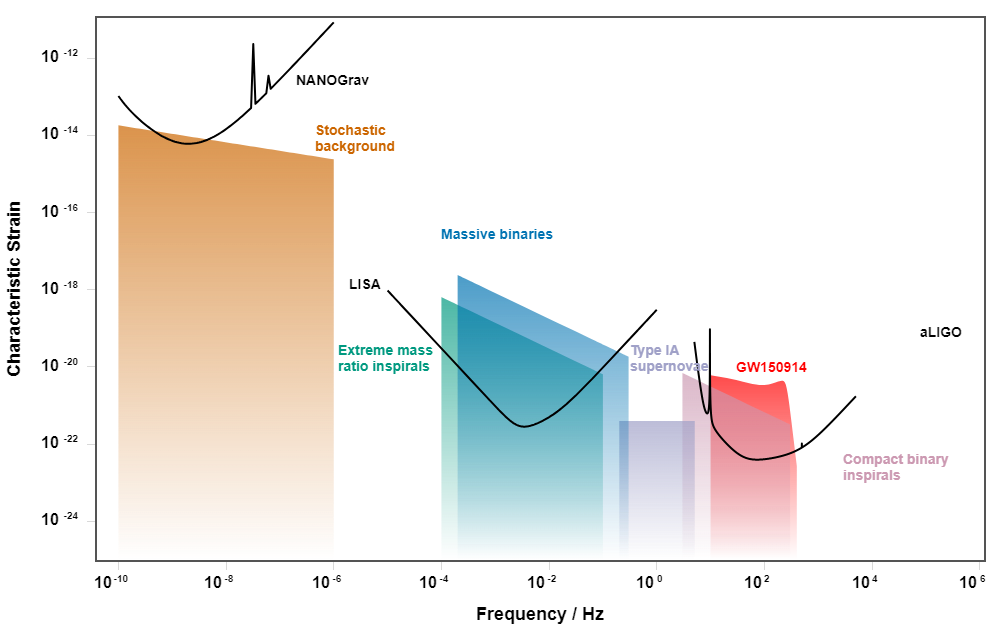
\includegraphics[width=\linewidth]{figs/my_gwplotter.png}
        \caption{Sensitivity Curve Example}
        \label{fig:sensitivity_curve}
    \end{figure}
\end{frame}

\section{Derivation of Quick Sensitivity Curves}

\begin{frame}{Quick Sensitivity Curve Derivation}
    We will start from the realistic sensitivity curves presented in eq. 92 of Hazboun et al. (2019),
    \[
    S_{\text{eff}}(f) = \left( \sum_I \sum_{J > I} \frac{T_{IJ}}{T_{\text{obs}}} \frac{\chi_{IJ}^2}{S_I(f) S_J(f)} \right)^{-1/2}
    \]
    \begin{itemize}
        \item $S_{\text{eff}}$ is the effective background sensitivity
        \item $T_{\text{obs}}$: Total observational time span
        \item $T_{IJ}$: Overlapping observational time span between pulsars $I$ and $J$
        \item $\chi_{IJ}$: correlation coefficients
        \item $S_I(f)$: Individual pulsar sensitivity $I$
    \end{itemize}
\end{frame}

\begin{frame}{Derivation of Quick Sensitivity Curves}
    Simplifying assumptions:
    \begin{itemize}
        \item Uniform distribution of pulsars across the sky
        \item Identical noise properties for all pulsars
        \item $T_I = T_{\rm obs}$ (all pulsars observed for full timespan)
        \item Same observational cadence for all pulsars
    \end{itemize}
\end{frame}

% Slide 5: Simplified Sensitivity Equation
\begin{frame}{Simplified Sensitivity Equation}
    Assuming uniform pulsar distribution across the sky,
    \[
    \chi_{IJ} \approx 1/48
    \]

    and identical noise properties:
    \[
    S_{\text{eff}}(f) = \left(\frac{N_{\rm psr}\left(N_{\rm psr}-1\right)}{2 \times 48 \times S_I(f)^2} \right)^{-1/2}
    \]
\end{frame}


\begin{frame}{Final Sensitivity Equation}
    From Equation 2, it follows that:
    \[
    S_{\text{eff}}(f) = \left(\frac{96}{N_{\rm psr}(N_{\rm psr}-1)}\right)^{1/2} \frac{12\pi^2f^2}{\mathcal{N}^{-1}_I(f)}
    \]
\end{frame}

\begin{frame}{Derivation of Quick Sensitivity Curves}
    \[
    S_{I}(f) = \frac{1}{\mathcal{N}_I^{-1}(f)\mathcal{R}(f)} = \frac{12\pi^2f^2}{\mathcal{N}_I^{-1}(f)}
    \]
    where $\mathcal{N}_I^{-1}(f)$ is the noise-weighted inverse transmission function for pulsar $I$.
\end{frame}

\begin{frame}{Noise-Weighted Inverse Transmission}
    \[
    \mathcal{N}^{-1}_I(f) \approx \frac{\mathcal{T}_I(f)}{P_{\rm N}(f)}
    \]
    where $\mathcal{T}_I(f) \approx \left(1 + \frac{1}{T_{\rm obs}f}\right)^{-6}$
\end{frame}

\begin{frame}{Noise Model}
    The power in the noise is given by:
    \[
    P_{N} = P_{\rm WN} + P_{\rm RN} = 2\Delta t\sigma^2 + A_{\rm RN}f^{-\gamma_{\rm RN}}
    \]
    where $\sigma$ is the time of arrival uncertainty, and $A_{\rm RN}$ models red noise.
\end{frame}

\section{Conclusion}
\begin{frame}{Conclusion}
    Accurate PTA sensitivity is expensive to compute.

    But with a few oversimplifications, we can get a quick estimate to characterize our detector.

\end{frame}

\begin{frame}{References}
    \begin{thebibliography}{1}
        \bibitem{Hazboun2019} Hazboun, J. S., Romano, J. D., Smith, T. L. (2019). Realistic sensitivity curves for pulsar timing arrays. \textit{Phys. Rev. D}, 100, 104028.
        \bibitem{Moore2015} Moore, C. J., Cole, R. H., Berry, C. P. L. (2015). Gravitational-wave sensitivity curves. \textit{Class. Quantum Grav.}, 32, 015014.
        \bibitem{Babak2024} Babak, S. et al. (2024). Forecasting PTA sensitivity. arXiv:2404.02864.
        \bibitem{Jennings2021} Jennings, R. (2021). Transmission Functions for Polynomial Fits. NANOGrav Memorandum 006.
    \end{thebibliography}
\end{frame}

\end{document}
